%---------- COURSE INFORMATION ------------------------
\newcommand{\course}{CIS 236-I01}
\newcommand{\coursetitle}{INFORMATION SYSTEMS IN ORGANIZATIONS}
\newcommand{\courseloc}{Online}
\newcommand{\coursetime}{Online}
\newcommand{\coursedesc}{A survey of information systems applications to support business processes, including operational, tactical, and strategic applications. Emerging and
pervasive hardware, software, telecommunications, and data resource management technologies are emphasized. Security, ethics, global/international aspects, and systems integration issues areconsidered using the information systems (IS) framework.}

\newcommand{\coursesec}{I01}
\newcommand{\coursecredithours}{3}
\newcommand{\courseprereq}{CIS 125 and one of the following: \\ & MA 110, 112, 113, 115, 125}
\newcommand{\coursedelmethod}{Online}

\newcommand{\courseobjectives}{\item Identify and define fundamental information systems concept
	\item Explain the impact of e-commerce and globalization on businesses
	\item Explain the significance of using systems analysis and design methods to solve problems faced by organizations
	\item Analyze personal, legal, ethical, and organizational issues of information systems
	\item Utilize business software applications to collect and analyze business data
	\item Summarize emerging trends in information systems and how they will shape the future of business organizations
	\item Develop a research paper relating to information systems that will include literature search, analysis, and recommendations
	\item Use appropriate information technology tools to develop a solution to a business-related problem
}

\newcommand{\coursetopics}{\item Usability of Interactive Systems
	\item Overview of information systems
	\item Computer hardware and software
	\item Database systems
	\item Personal, legal, ethical, and organizational issues
	\item Protecting information resources
	\item Data communications
	\item Internet and web applications
	\item E-Commerce 
	\item Global information systems
	\item Building successful information systems 
	\item Emerging trends, technologies, and applications}
\newcommand{\coursegrades}{Subject Exams\dotfillsmall 30\% \\
		Quizzes\dotfillsmall 10\% \\
		Research Paper\dotfillsmall 10\% \\
		Discussions\dotfillsmall 15\% \\
		Other Assignments\dotfillsmall 35\%}
\newcommand{\coursetext}{
	\adjustbox{valign=c}{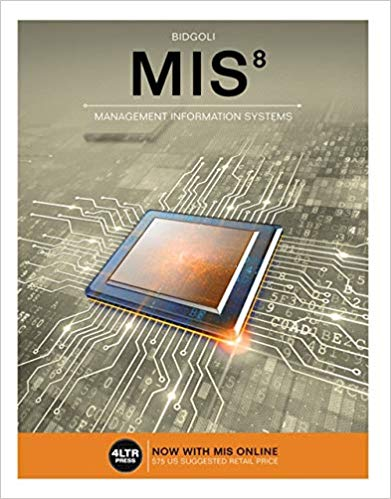
\includegraphics[width=1in]{img/cis236ed8}} & \hangindent .4in \textbf{Textbook:} Bidgoli, H., MIS 8 (8th Edition). Cengage Learning. ISBN-10: 1337406929, ISBN-13: 978-1337406925. \\
	%& \hangindent .4in Simulation Software: SAM 365 \& 2016 Assessments, Trainings, and Projects with MindTap Reader.
}
